\chapter{ANEXO A}\label{anexoa}

Fazendo uma análise do pacote \textit{bluetooth}, existe a classe \textit{BluetoothConnection} que traz um método estático chamado \textit{getConnectionBluetooth} (Figura \ref{Fig:get_connection_bluetooth}), esperando como parâmetro uma URL de conexão. Este método que tem a responsabilidade de obter uma conexão \textit{bluetooth} devolvendo um objeto do tipo \textit{StreamConnection}, pertencente à biblioteca \textit{BlueCove}. A Classe \textit{DiscoveryDevices} (Figura \ref{Fig:discovery_devices}) implementa a interface \textit{DiscoveryListener}, também pertencente à biblioteca \textit{BlueCove}, que permite a descoberta de dispositivos e serviços. Esta interface fornece quatro métodos para serem implementados: dois para descobrir dispositivos, que são o \textit{deviceDiscovered} (Figura \ref{Fig:device_discovered}) – método que é invocado quando é encontrado um dispositivo durante uma consulta – e o \textit{inquiryCompleted} (Figura \ref{Fig:inquiry_completed}) – método que é chamado quando uma consulta é concluída, e dois para descobrir serviços, que são o \textit{servicesDiscovered} (Figura \ref{Fig:services_discovered}) – são invocados quando os serviços são encontrados durante uma pesquisa por serviços – e o \textit{serviceSearchCompleted} (Figura \ref{Fig:service_search_completed}) – são chamados quando uma pesquisa de serviço foi concluída ou encerrada devido a um erro \cite{bluecovedoc}. Além destes métodos contidos na assinatura da interface, a classe \textit{DiscoveryDevices} também traz o método \textit{discovery} (Figura \ref{Fig:discovery}), responsável por iniciar a descoberta de dispositivos.

\begin{figure}[!ht]
\centering
\caption{Foto do método \textit{getConnectionBluetooth} da classe \textit{BluetoothConnection}.} 
{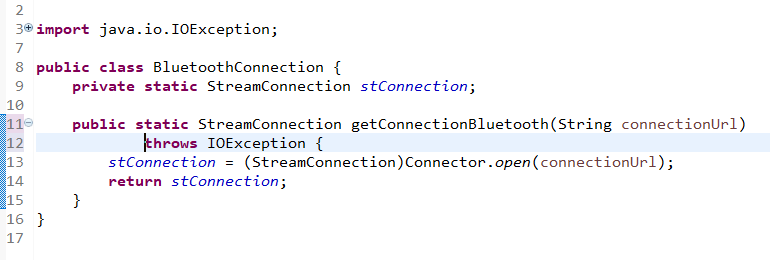
\includegraphics[scale=.80]{imagens/pacoteBluetooth-BluetoothConnection.PNG}}\\
\makebox[\width]{Fonte: produzido pelo autor} \label{Fig:get_connection_bluetooth}
\end{figure}

\begin{figure}[!ht]
\centering
\caption{Foto da Classe \textit{DiscoveryDevices} implementando a interface \textit{DiscoveryListener}.} 
{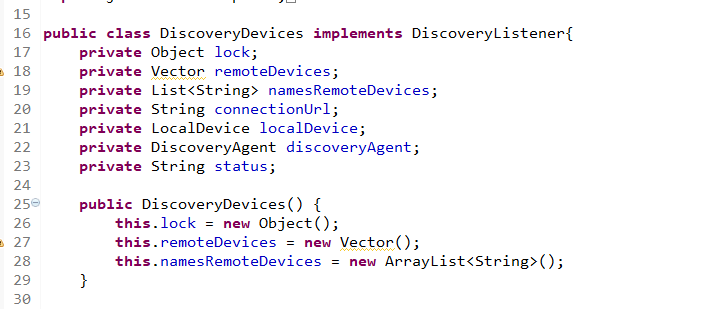
\includegraphics[scale=.94]{imagens/pacoteBluetooth-DiscoveryDevices_DiscoveryListener.PNG}}\\
\makebox[\width]{Fonte: produzido pelo autor} \label{Fig:discovery_devices}
\end{figure}

\begin{figure}[!ht]
\centering
\caption{Foto do método \textit{deviceDiscovered} da classe \textit{DiscoveryDevices}.} 
{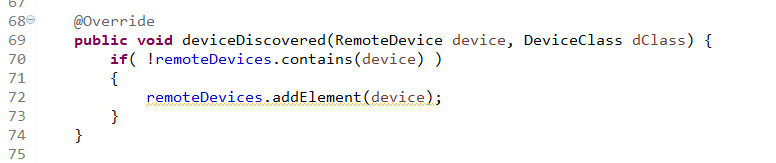
\includegraphics[scale=.78]{imagens/pacoteBluetooth-DiscoveryDevices_deviceDiscovered.PNG}}\\
\makebox[\width]{Fonte: produzido pelo autor} \label{Fig:device_discovered}
\end{figure}

\begin{figure}[!ht]
\centering
\caption{Foto do método \textit{inquiryCompleted} da classe \textit{DiscoveryDevices}.} 
{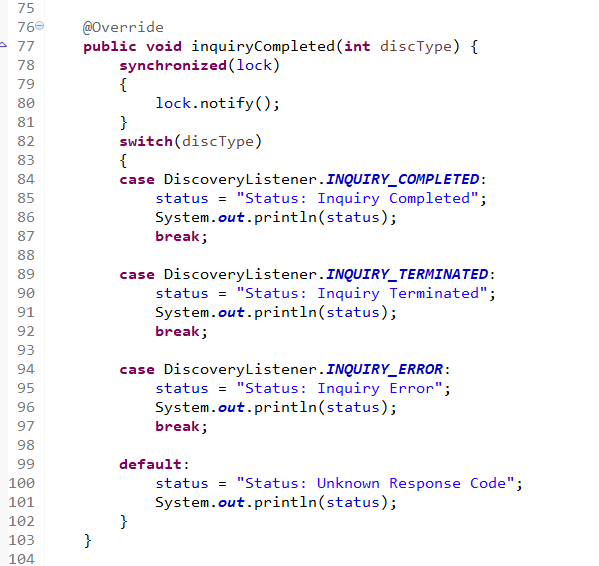
\includegraphics[scale=.80]{imagens/pacoteBluetooth-DiscoveryDevices_inquiryCompleted.PNG}}\\
\makebox[\width]{Fonte: produzido pelo autor} \label{Fig:inquiry_completed}
\end{figure}

\begin{figure}[!ht]
\centering
\caption{Foto do método \textit{servicesDiscovered} da classe \textit{DiscoveryDevices}.} 
{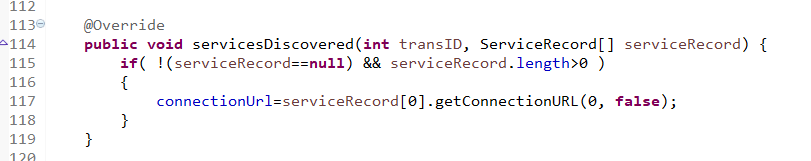
\includegraphics[scale=.78]{imagens/pacoteBluetooth-DiscoveryDevices_servicesDiscovered.PNG}}\\
\makebox[\width]{Fonte: produzido pelo autor} \label{Fig:services_discovered}
\end{figure}

\begin{figure}[!ht]
\centering
\caption{Foto do método \textit{serviceSearchCompleted} da classe \textit{DiscoveryDevices}.} 
{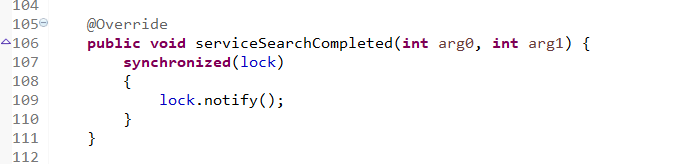
\includegraphics[scale=.78]{imagens/pacoteBluetooth-DiscoveryDevices_serviceSearchCompleted.PNG}}\\
\makebox[\width]{Fonte: produzido pelo autor} \label{Fig:service_search_completed}
\end{figure}

\begin{figure}[!ht]
\centering
\caption{Foto do método \textit{discovery} da classe \textit{DiscoveryDevices}.} 
{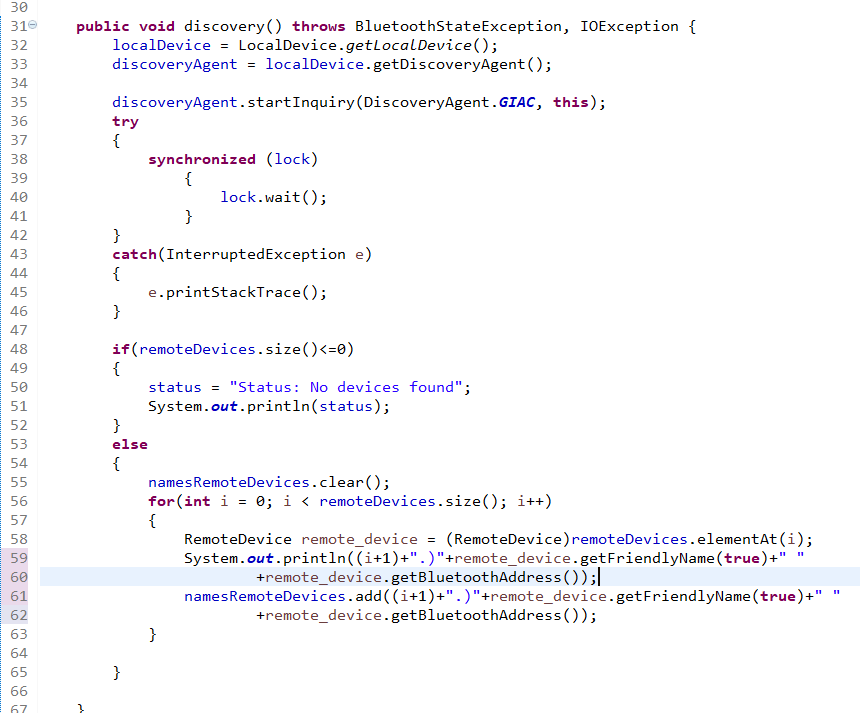
\includegraphics[scale=.70]{imagens/pacoteBluetooth-DiscoveryDevices_discovery.PNG}}\\
\makebox[\width]{Fonte: produzido pelo autor} \label{Fig:discovery}
\end{figure}

Observando o pacote \textit{scanner}, existe a classe \textit{ConnectToDevice} (Figura \ref{Fig:connect_to_device}) que espera como parâmetro em seu construtor um objeto do tipo \textit{DiscoveryDevices}. Esta classe também possui o método \textit{connectToDevice} (Figura \ref{Fig:connect_connect_to_device}), que espera como parâmetro um índice referente ao dispositivo que se deseja conectar. 

\begin{figure}[!ht]
\centering
\caption{Foto da classe \textit{ConnectToDevice}.} 
{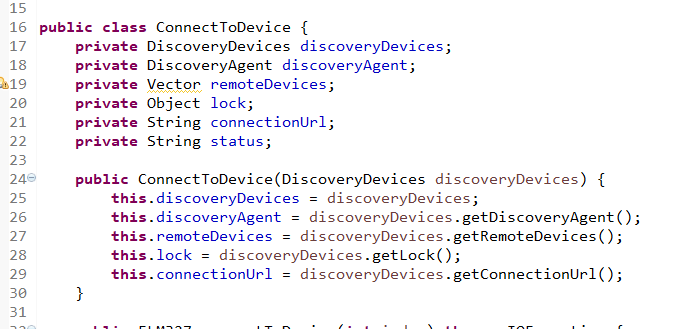
\includegraphics[scale=.80]{imagens/pacoteScanner-ConnectToDevice.PNG}}\\
\makebox[\width]{Fonte: produzido pelo autor} \label{Fig:connect_to_device}
\end{figure}

\begin{figure}[!ht]
\centering
\caption{Foto do método \textit{connectToDevice} da classe \textit{ConnectToDevice}.} 
{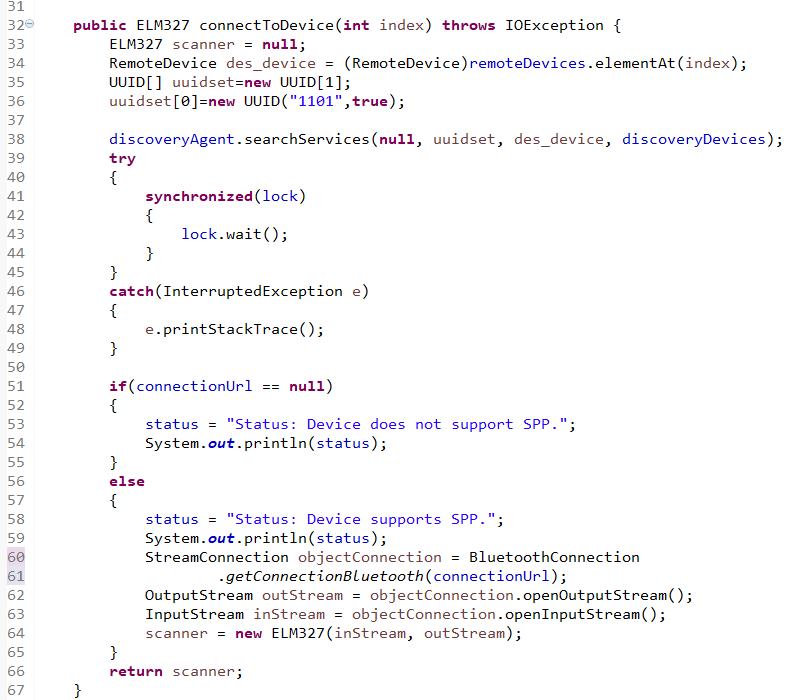
\includegraphics[scale=.70]{imagens/pacoteScanner-ConnectToDevice_connectToDevice.PNG}}\\
\makebox[\width]{Fonte: produzido pelo autor} \label{Fig:connect_connect_to_device}
\end{figure}